\chapter{Ensamblaje e instrumentacion}

En este capitulo se presentaran todos los detalles del ensamblado del reflector parabolico, la instalacion del rotor y la integracion de estos con el soporte de la montura en el pedestal construido para el telescopio. Tambien se detallaran todos los instrumentos evaluados y seleccionados para la construccion del receptor de radiofrecuencia, el rack de control y la infraestructura de caracterizacion.\\

Junto con esto, se mosntraran todas las piezas diseñadas e impresas en 3D para el soporte del alimentador y todos los soportes especificos que se necesitaron para la instalacion de los distintos componentes del telescopio.\\

Para finalizar con la descripcion del software creado para la operacion, mantenimiento y caracterizacion del telescopio.\\

\section{Ensamblado Mecánico}

Tanto el reflector parabolico como la montura alt azimutal y su correspondiente controlador, son elementos adquiridos de la compañia \textit{RFHamdesign}, una empresa holandesa que se especializa en la construccion de telescopios de radio aficionados. El reflector de 3 metros venia completamente desarmado y con piezas que requerian ser modificadas y ensambladas para su correcto funcionamiento.\\

Para todo el ensamblado se utilizaron herramientas de y electricas, como taladors, tijeras de ojalata, remachadoras, etc.\\

\begin{figure}
    \centering
    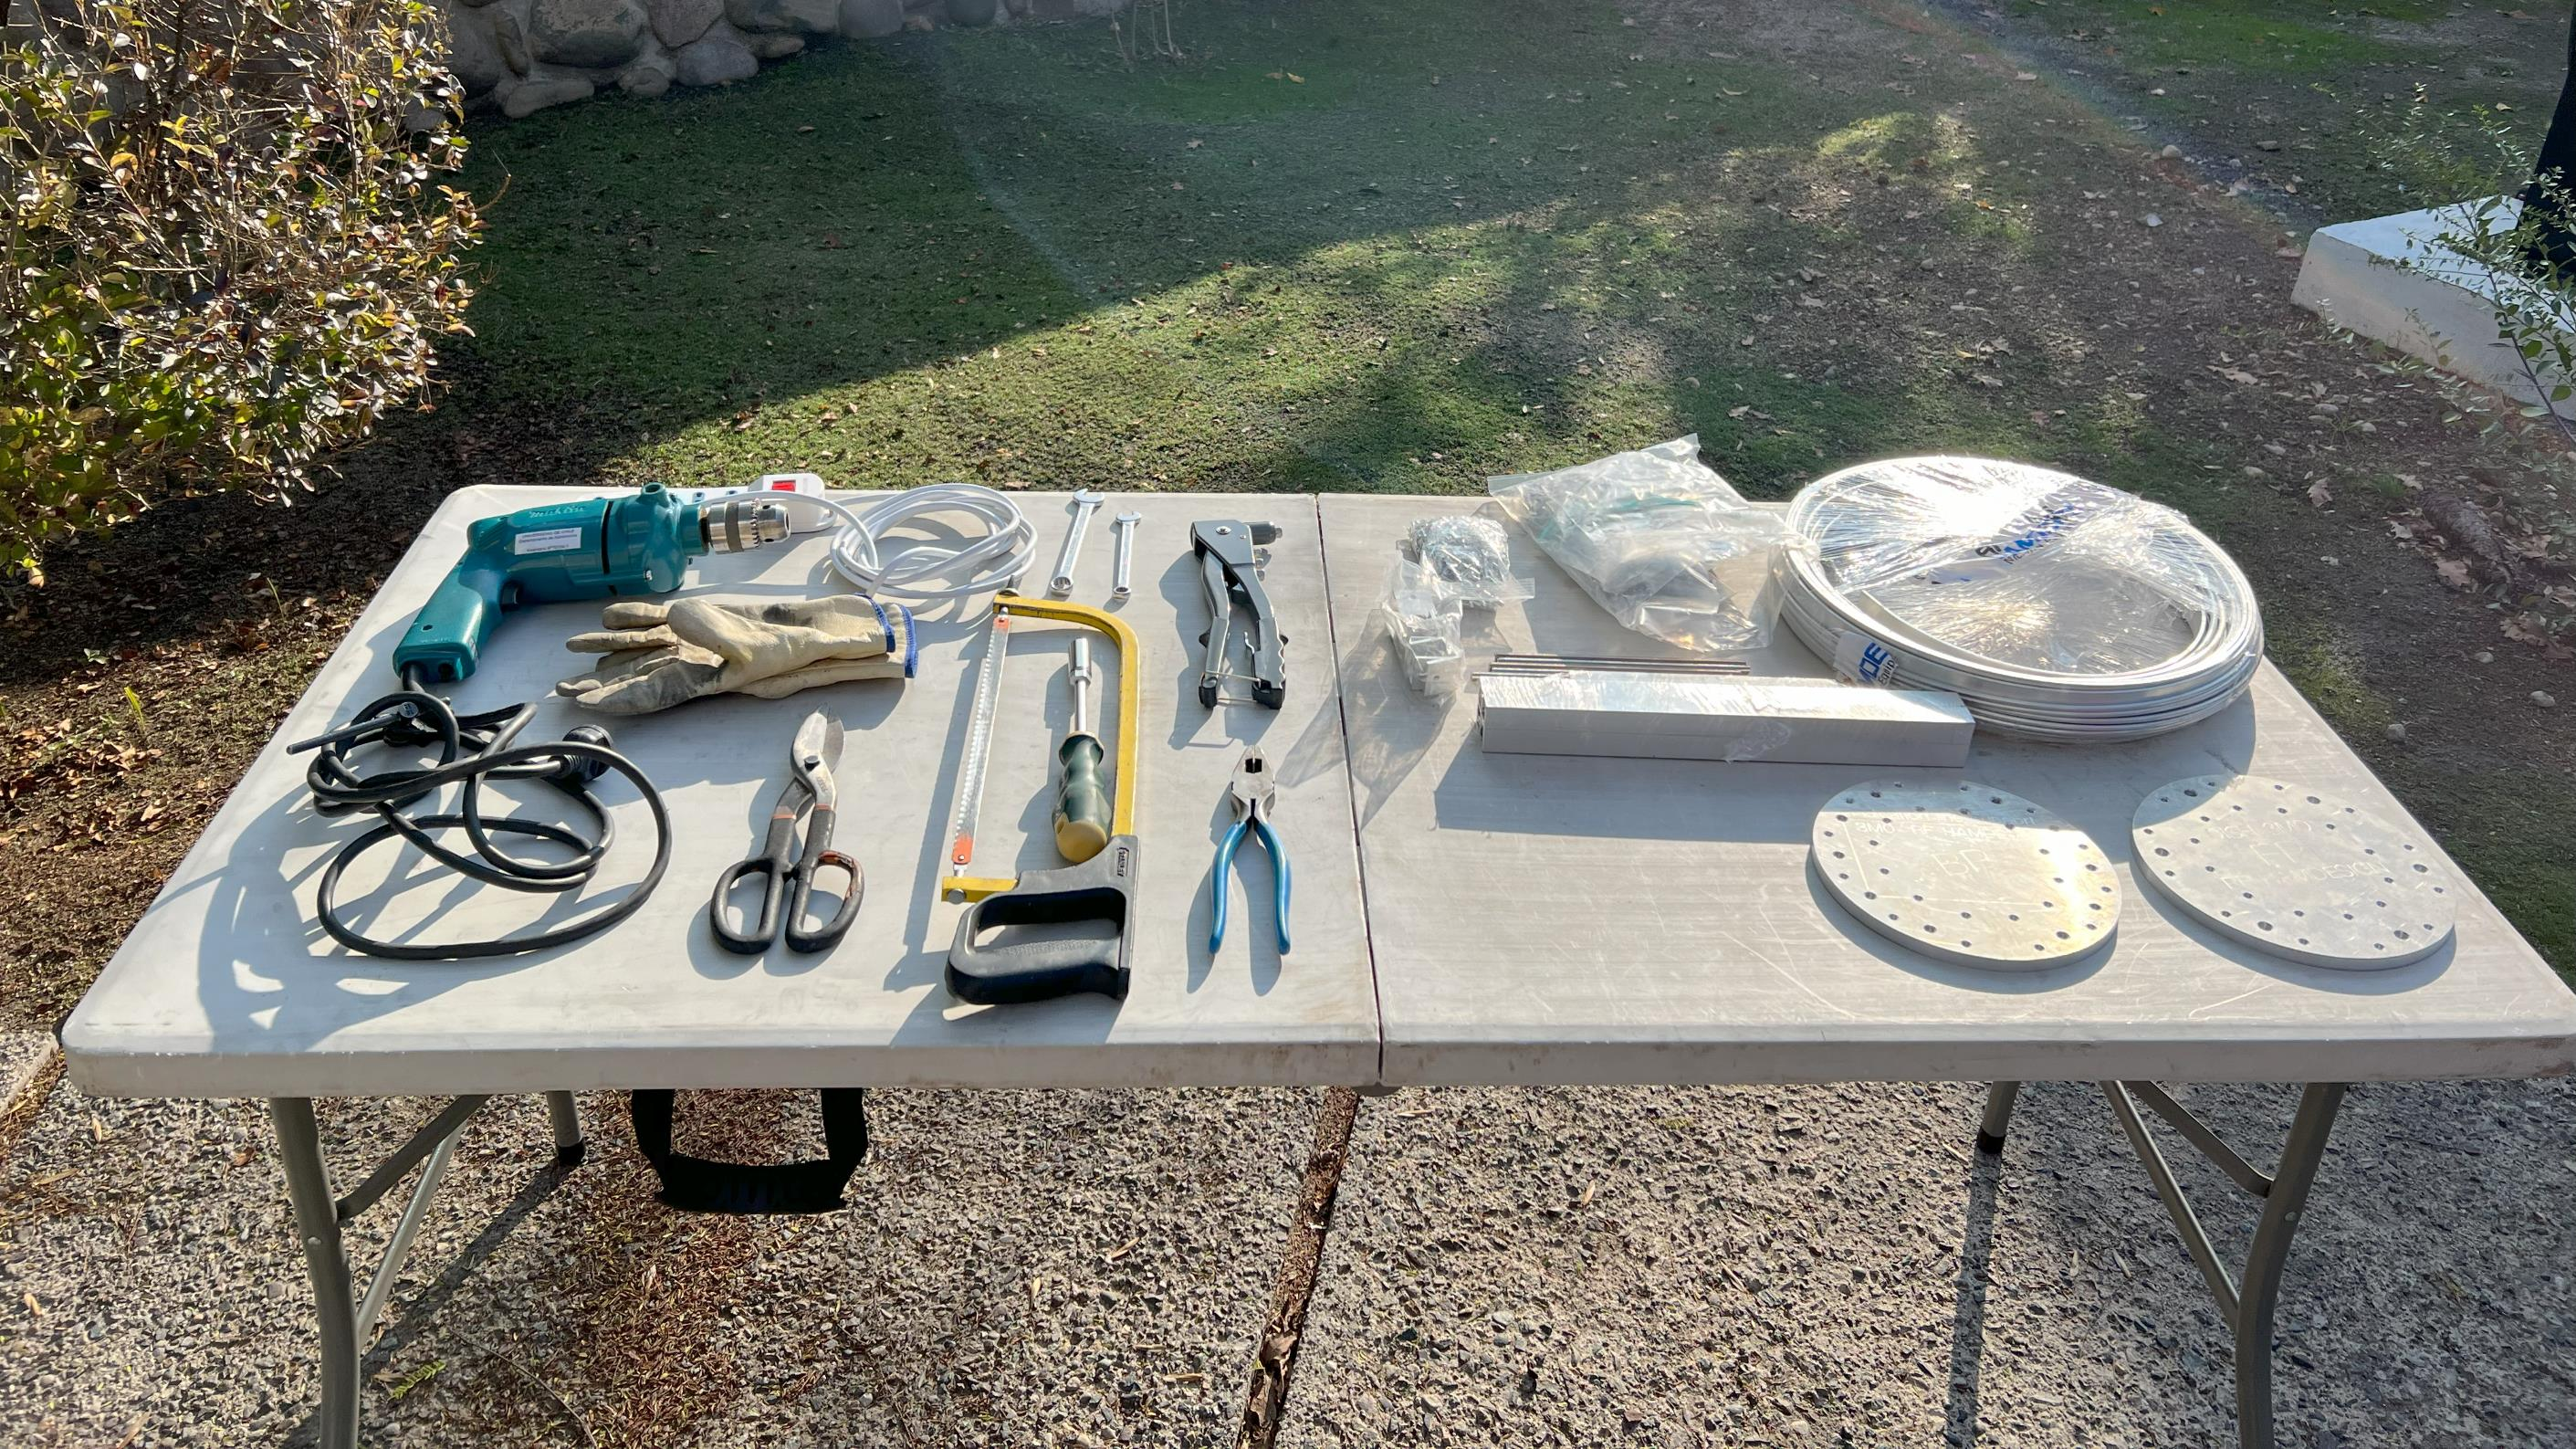
\includegraphics[width=0.8\textwidth]{img/herramientas}
    \caption{Herramientas utilizadas para el ensamblado de la superficie del reflector parabólico.}
    \label{fig:ensamblado1}
\end{figure}

En la figura \ref{fig:ensamblado1} se pueden ver las herramientas utilizadas para el ensamblado de la superficie del reflector parabólico ademas de las piezas que requerian de modificacion adicional para la instalacion correcta.\\

\subsection{Reflector Parabólico}

Las piezas del reflector se dividen en los 12 arcos, o costillas, de aluminio que conforman la estructura que da forma a la superficie parabolica, con un centro de aluminion donde estas 12 piezas se unen y apernan.\\

\begin{figure}
    \centering
    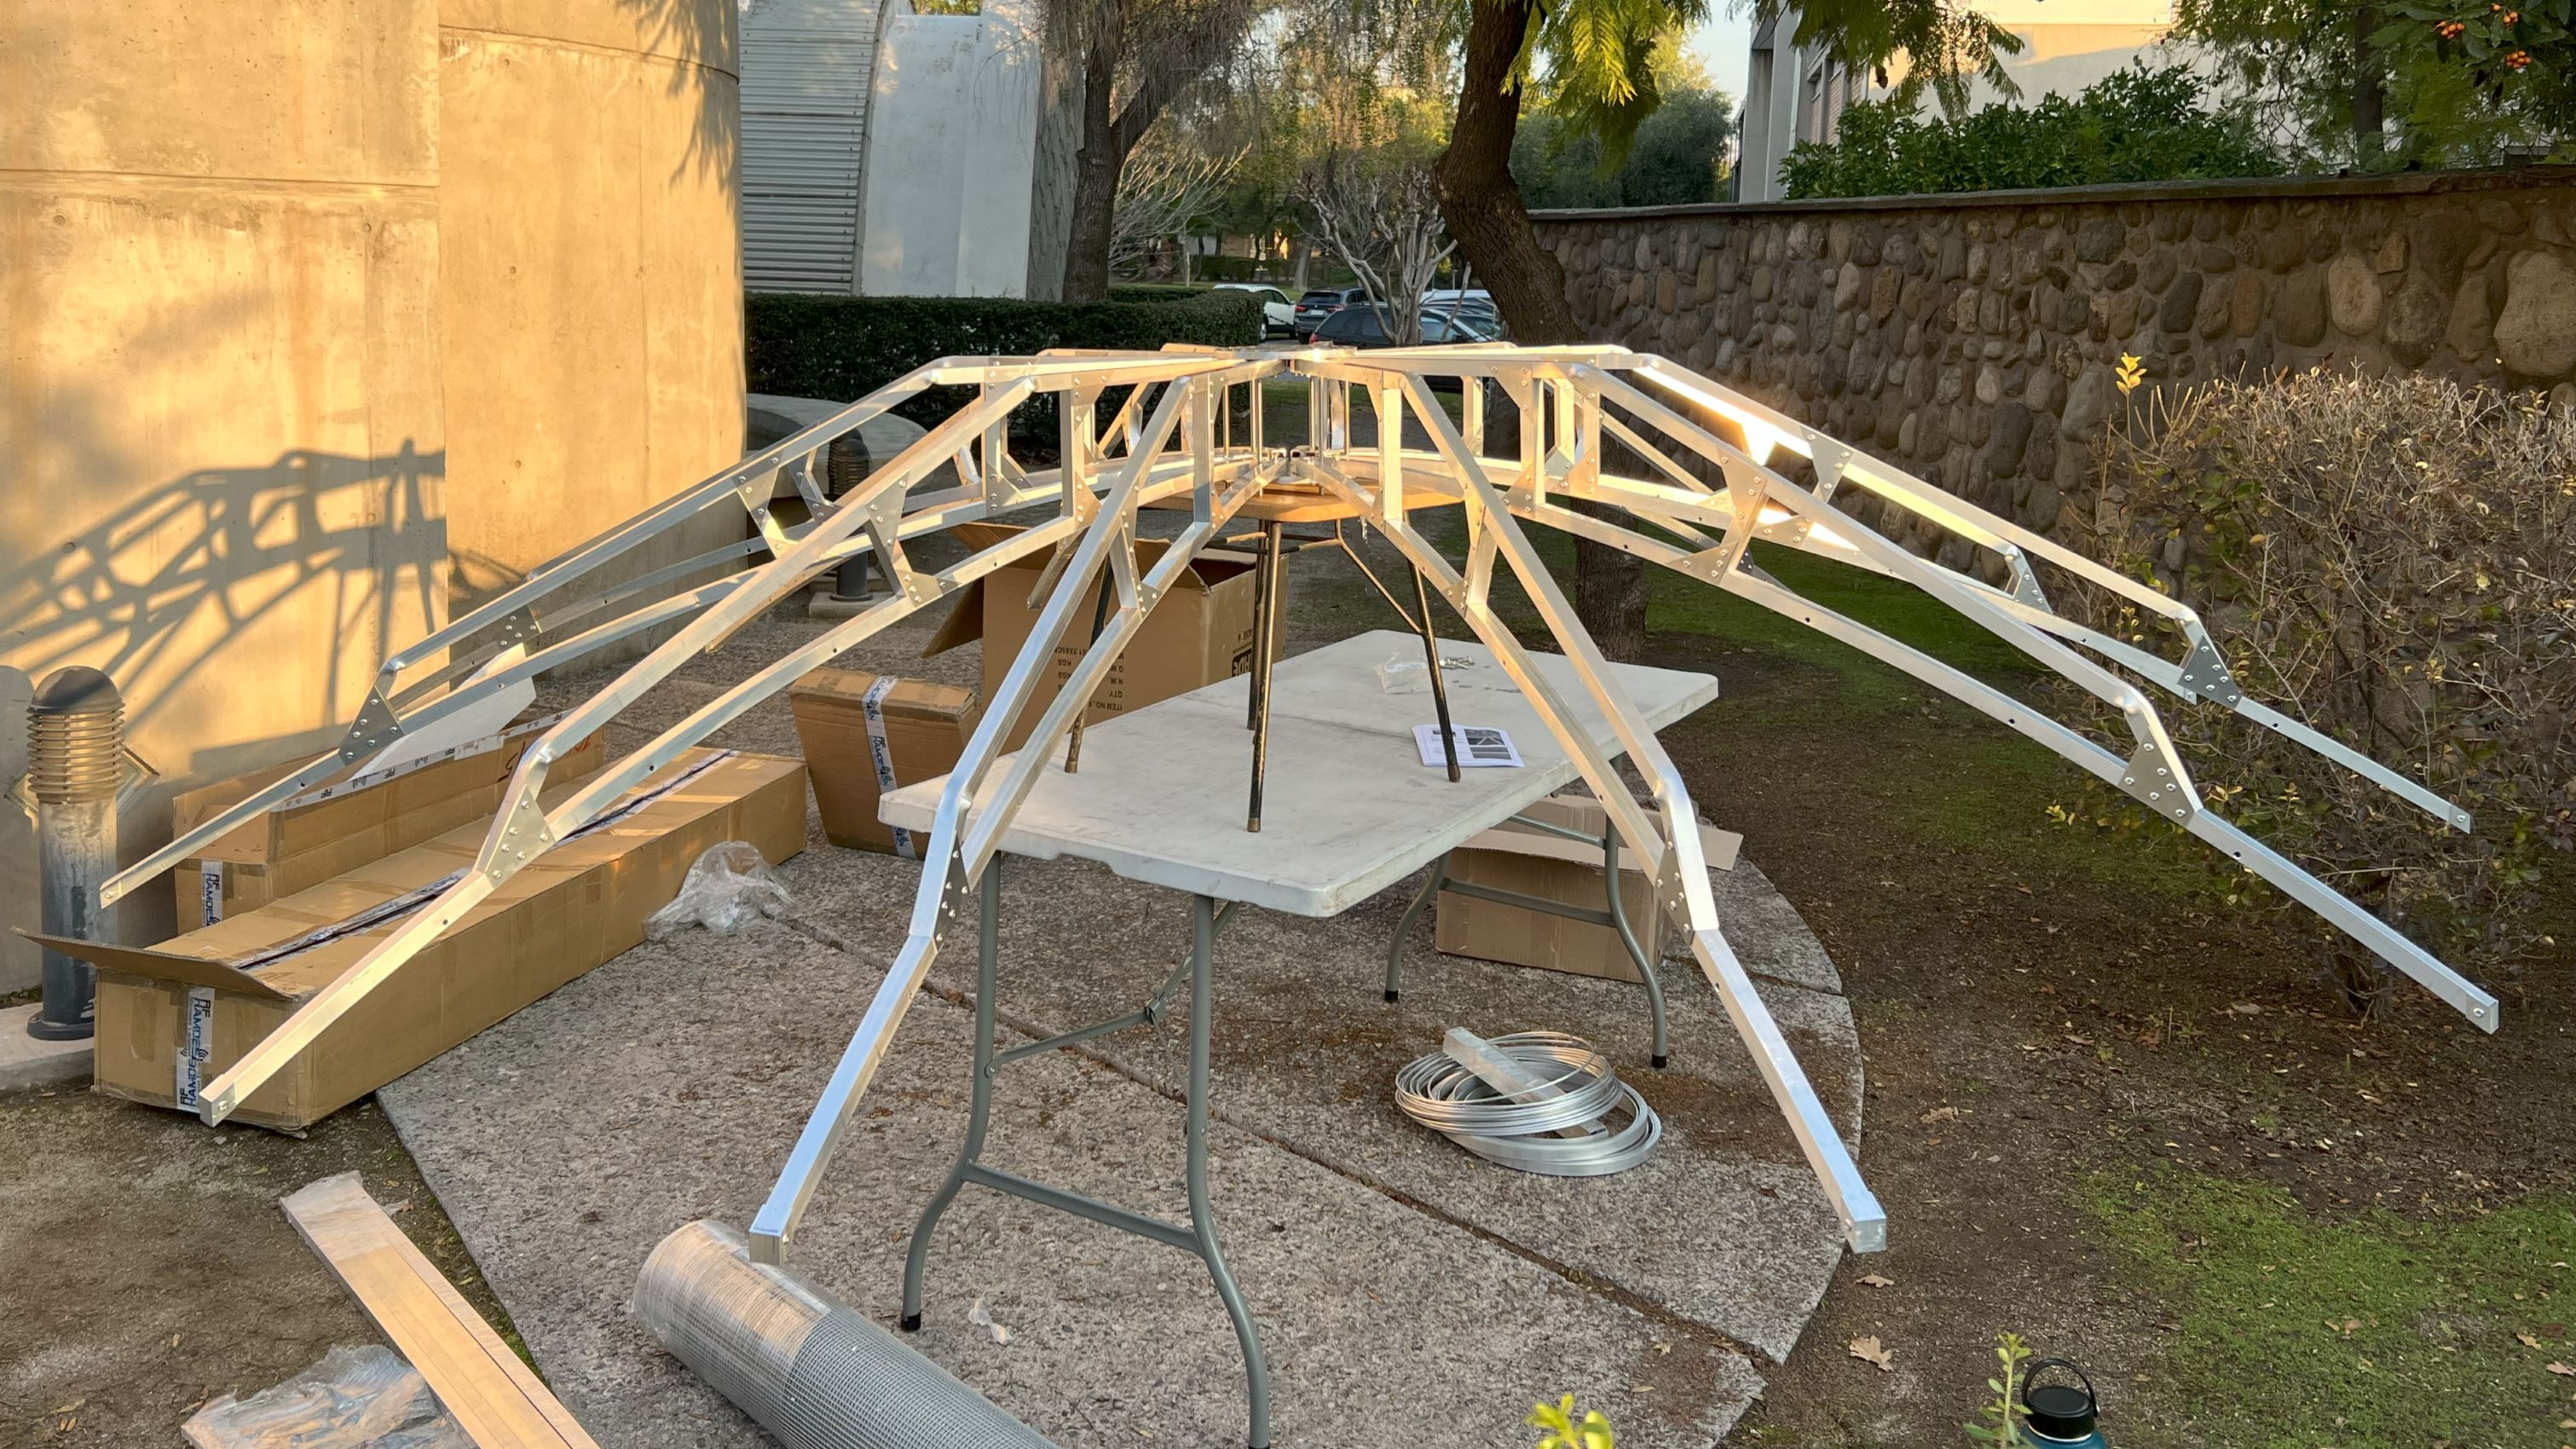
\includegraphics[width=0.8\textwidth]{img/estructura1}
    \caption{Los 12 arcos de alumunio apernados al centro del reflector parabólico.}
    \label{fig:ensamble2}
\end{figure}

En la figura \ref{fig:ensamble2} se pueden ver los 12 arcos de aluminio apernados a los discos de distribucion, que ademas es el punto de anclaje para el soporte de la montura.\\

Luego desenrollan y enderezan los tubos de aluminio que confirmar los anillos donde se tensaeran las mallas metalicas que conforman la superficie del reflector. Con la misma logica se toma la cinta de alumninio, que es aproximadamente de 4 mm de espesor, para enderesarla y prepara las perforaciones para los primeros remaches.\\

\begin{figure}
    \centering
    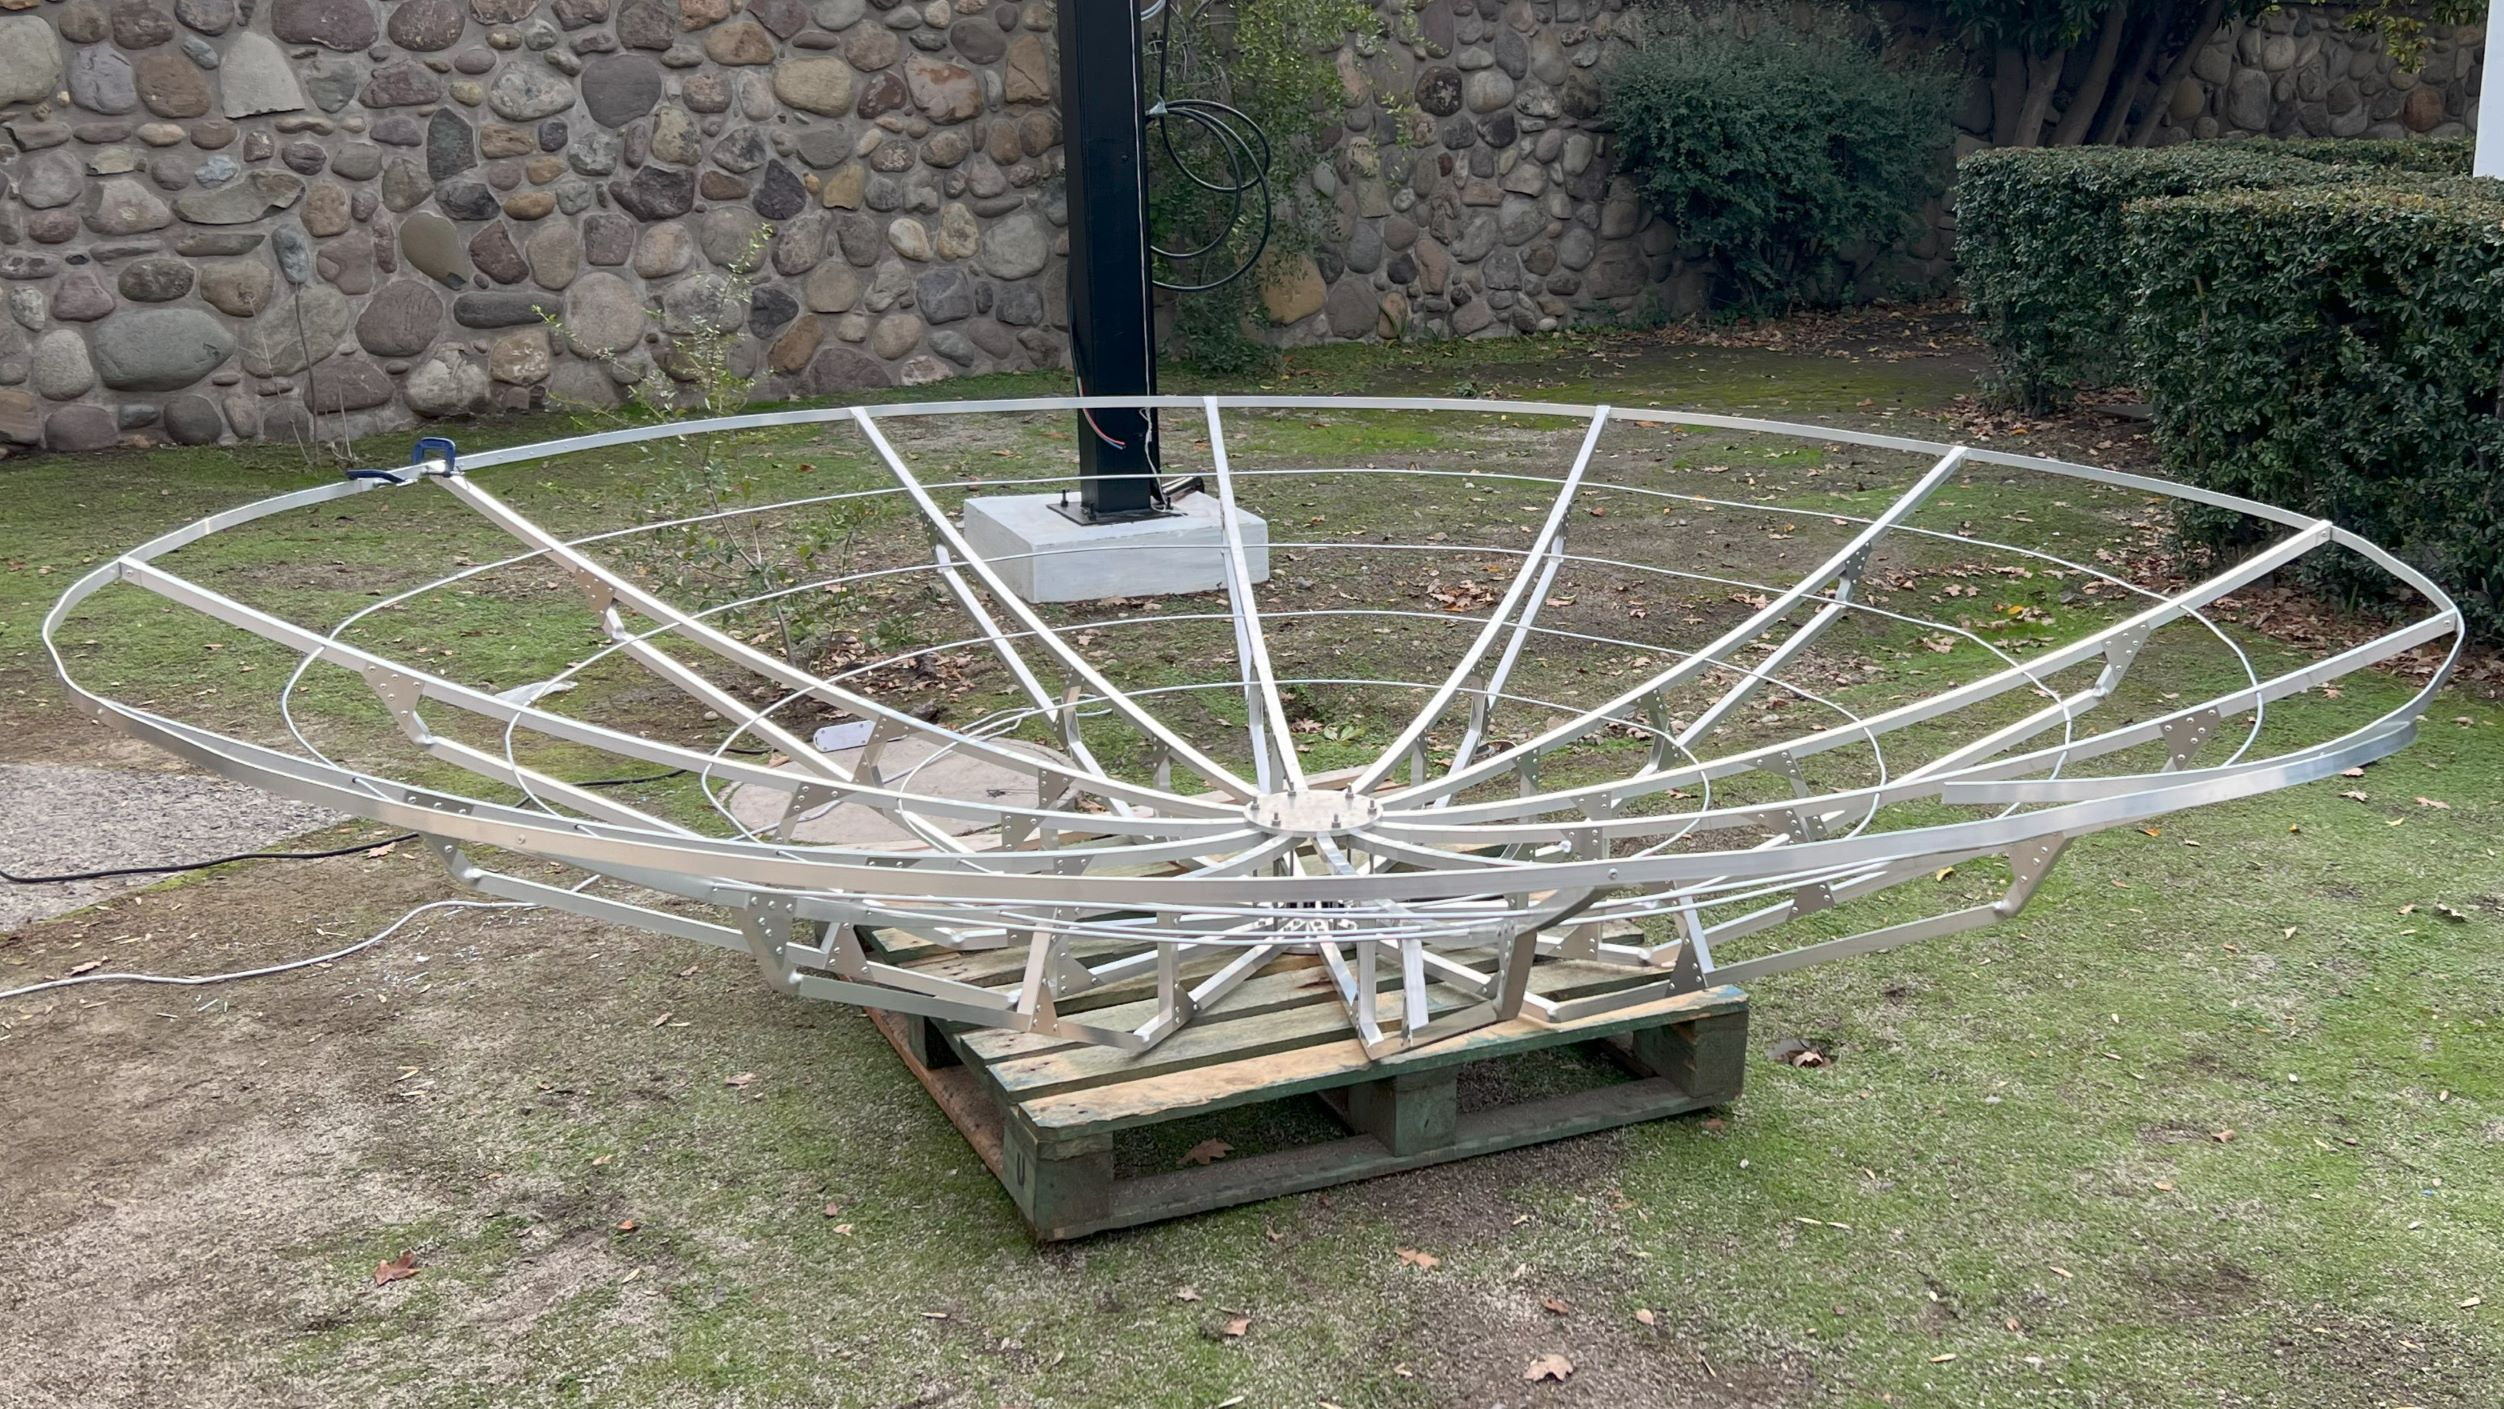
\includegraphics[width=0.8\textwidth]{img/estructura2}
    \caption{Los tubos de aluminio y la cinta de aluminio para la tensión de la malla metálica instalados radialmente en los soportes.}
    \label{fig:ensamble3}
\end{figure}

\subsection{Diseño de soportes adicionales}

Para poder instalar todos los componentes del telescopio, se debian fabricar soportes personalizados y adicionales para así poder utilizar receptores y elementos que no fueran parte del kit original del fabricante. Con el objetivo de reducir los timepos de fabricación y prototipado al usar componentes de aluminio o acero se decidio utilizar impresion 3D con filamento plastico PLA\footnote{Explicacion PLA} de alta resistencia mecanica.\\

Se diseñaron 6 piezas en total con el software de diseño asistido por computadora o \textit{CAD} \textit{Fusion 360} de la compañia \textit{Autodesk}. Todos los comonentes fueron impresos en PLA de alta resistencia o \textit{Hyper-PLA} de la compañia \textit{Creality}, otorgando una mayor resitencia a la flexion de 50\% que el PLA convencional y una elongacion de 6.304\% en comparacion con la del PLA convencional de 3\%. La configuracion de la impresion fue una altura de capa de 0.2 mm, dada por la boquilla utilizada, 4 capas de muralla y un \textit{Infill} o relleno de 60 \%.\\

Una ventaja importante en la elección de la impresion 3D en filamentops plasticos, es su baja incidencia en la deformacion o interferencia del comportamiento de radiofrecuencia, al ser un material no conductor introducido en el campo cercano de los componentes.\\

\begin{figure}
    \centering
    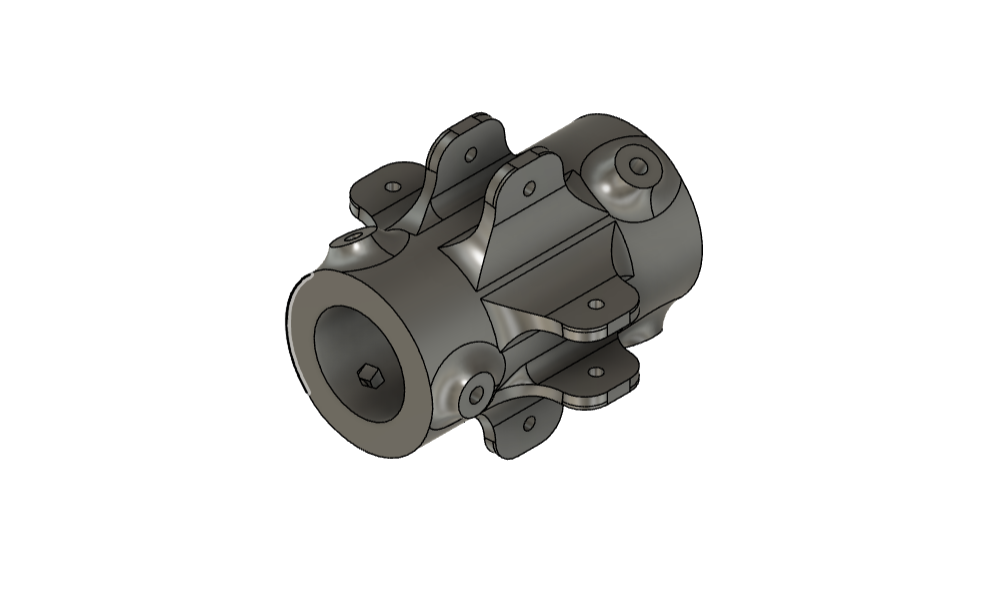
\includegraphics[width=0.8\textwidth]{img/soporte3D5}
    \caption{Union de los doportes de aluminio para el alimentador}
    \label{fig:ensamble4}
\end{figure}

El diseño 3D de la figura \ref{fig:ensamble4} es un soporte que contiene una cabidad centrar cilindrica que conmple la funcion de sostener tanto el alimentador como el receptor por medio de un tubo plastico de PVC\footnote{PVC} que asegura que todo se mantenga alineado con el centro de la parabola, además de permitir un movimiento en el eje de la cabidad cilindrica para ajustar el foco del alimentador.\\

Tiene también 4 ranuras perforadas para aseguirar los soportes con pernos M4 de medida y también 6 perforaciones con cabidades para tuercas M5. Con estas tuercas y con los respectivos tornillos se asegura la poscision del tubo de PVC para fijar el foco una vez encontrado.\\

Las siguientes piezas comparten la misma filosofia de diseño, para poder compatible entre ellas y con el resto de los componentes del telescopio. Además, permiten el rediseño de nuevas piezas para otros alimentadores, cambios de largo en el tubo distriubidor de PVC y en la eleccion de otro material de impreson 3D si se quiciese.\\

\begin{figure}
    \centering
    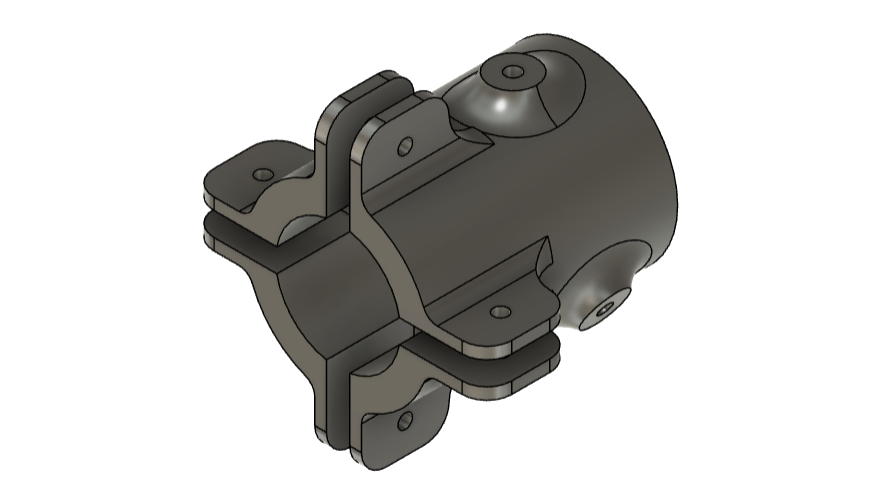
\includegraphics[width=0.8\textwidth]{img/soporte3D1v1}
    \caption{Interfaz de soporte para el tubo de distribucion y otros elementos}
    \label{fig:ensamble5}
\end{figure}

La figura \ref{fig:ensamble5} es un soporte multiproposito que permite acoplar otros soportes de menor complejidad para ser instalados en la zona del alimentador y receptor. Así permite cambios radicales en la instrumentación que se requiera en el futuro sin tener que rediseñar toda la estructura de sujeción.\\

\begin{figure}
    \centering
    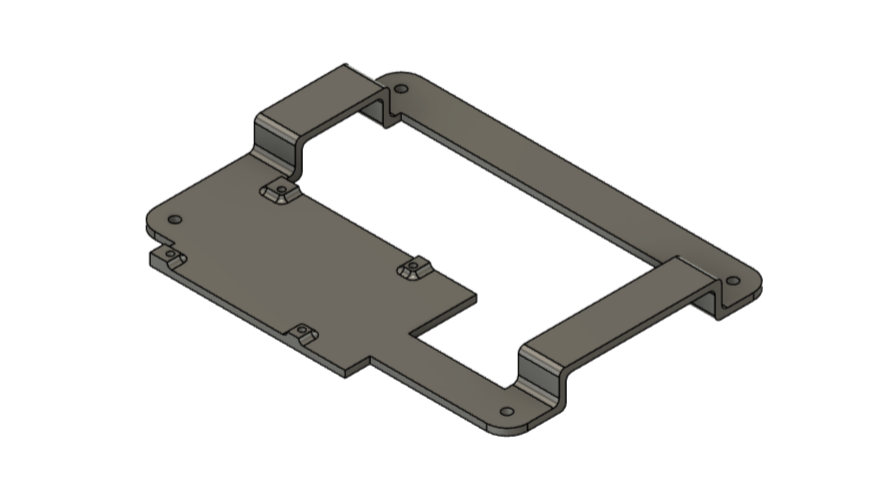
\includegraphics[width=0.8\textwidth]{img/soporte3D7}
    \caption{Soporte interno para electronica de recepción}
    \label{fig:ensamble6}
\end{figure}

El receptor de radiofrecuencia se encuentra dentro de una caja electrica a prueba de agua, pero se requiere un soporte interno para asegurar que la placa de adquisicion de datos y el digitalizador no se muevan y se mantengan en su lugar mientras el telescopio se mueve en distintas elevaciones. La figura \ref{fig:ensamble6} es un soporte que se instala en la caja electrica y permite montar diferentes tipos de receptores y amplificadores.\\


\subsection{Montura Alt-Azimutal}

\subsection{Rack de control}

\section{Alimentador}

\section{Diseño del receptor}

\subsection{Cadena de recepción}

\subsection{Digitalizador y adquisición}

\section{Software de control y adquisición}

\subsection{Control de la montura}

\subsection{Adquisición de datos}

\section{Infraestructura de caracterizacion}

\subsection{Fuente de calibración}

\subsection{Fuente de ruido}

\subsection{Software de caracterización}